\chapter{Erster Ansatz: Bitcoin}
\label{btc}

\section{Grundlagen}
Bei Bitcoin handelt es sich um die erste digitale, dezentral organisierte Währung. Die Idee digitaler Währungen existiert bereits seit der Erfindung des Internets. Allerdings scheiterten diese in der Vergangenheit daran, dass sie auf einen zentralen Punkt der Kontrolle angewiesen waren und somit einen Single Point of Failure beinhalteten. Die am 03. Januar 2009 gestartete digitale Währung ''Bitcoin'' schaffte es erstmalig gänzlich auf die Verwendung einer zentralen Instanz zu verzichten und somit ein verteiltes, dezentrales und sicheres digitales Zahlungssystem zu realisieren. Bitcoin wurde in dem von dem Pseudonym ''Satoshi Nakamoto'' veröffentlichen Paper ''Bitcoin: A Peer-to-Peer Electronic Cash System'' das erste Mal beschrieben. \if Der Source Code der Bitcoin Software ist öffentlich verfügbar und hat dadurch seit 2009 eine regelrechte Innovationsexplosion im Bereich der digitalen Währungen ausgelöst.\fi Bitcoin funktioniert durch das Zusammenspiel mehrerer Komponenten und besteht aus:

\begin{itemize}
\item Einem dezentralen Peer-to-Peer Netzwerk, dass mit Hilfe des Bitcoin-Protokolls kommuniziert.
\item Der Blockchain, die eine öffentlichen Transaktionsdatenbank darstellt, die alle validen Transaktionen seit dem Start des Netzwerkes aufzeichnet.
\item Eine Menge an Konsensregeln mit Hilfe derer Netzwerkteilnehmer eigenständig Transaktionen auf ihre Richtigkeit prüfen können.
\item Ein Proof-of-Work Algorithmus der es erlaubt, sich in dem globalen dezentralen Netzwerk auf den Zustand der Transaktionsdatenbank zu einigen. Das kontinuierliche Ausführen des Proof-of-Work Algorithmus wird ''Mining'' genannt.
\end{itemize}

\subsection{Peer-to-Peer Netzwerk}
Peer-to-Peer-Netzwerke sind Netzwerke, die auf direkten Verbindungen zwischen Rechnern beruhen, ohne dass dabei einer der Rechner eine Sonderstellung einnimmt oder ein Server die Kommunikation vermittelt. In einem reinen Peer-to-Peer-Netz sind alle Computer gleichberechtigt und können sowohl Dienste in Anspruch nehmen, als auch zur Verfügung stellen. Das Peer-to-Peer-Modell ist somit grundlegend verschieden von dem im Internet am häufigsten verwendeten Client-Server-Modell. Da jeder Knoten des Netzwerks gleichzeitig Client und Server ist, gibt es keine zentrale Instanz die einen sogenannten ''Single Point of Failure'' darstellt. 

\begin{figure}[H]
\centering
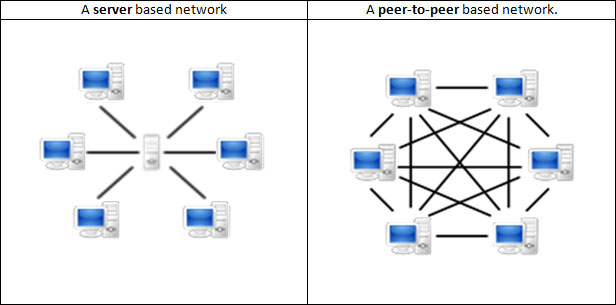
\includegraphics[width=1\linewidth]{Figures/p2p_networks}
\decoRule
\caption{Client-Server | Peer-to-Peer \cite{wikipedia_p2p}}
\label{fig:p2p_networks}
\end{figure}

Peer-to-Peer Netzwerke sind selbstorganisierend. Das Hinzufügen neuer Teilnehmer und das Entfernen bestehender Netzwerkknoten findet ohne eine zentrale Verwaltung statt und behindert die Funktionsweise des Netzwerks nicht. Jeder Knoten des Netzwerks verwaltet eigenständig seine direkten Nachbarknoten. Die Art und Weise wie die Teilnehmer des Netzwerkes miteinander Kommunizieren ist durch das Netzwerkprotokoll vorgegeben. Um am Netzwerk teilzunehmen braucht man nur eine Software, die das Netzwerkprotokoll implementiert und einen Internetanschluss. Im Falle der Kryptowährungen nennt man die Software ''Wallet'' (englisch für Brieftasche), da man mit ihr Zahlungen initiieren und empfangen kann. Möchte ein Teilnehmer Bitcoins an einen anderen Teilnehmer senden, erstellt er dazu eine Nachricht die solch eine Transaktion beinhaltet und schickt sie an seine direkten Nachbarn des Peer-to-Peer Netzwerks. Die Nachbarn prüfen die Gültigkeit der Transaktion leiten diese gegebenenfalls an ihre Nachbarn weiter. Auf diese Art und Weise verteilt sich eine Transaktion im gesamten Netzwerk.


\subsection{Blockchain}
Eine Blockchain ist eine global verteilte Transaktionsdatenbank. Jeder Teilnehmer des Peer-to-Peer Netzwerkes speichert lokal eine Kopie dieser Datenbank. Dies erlaubt es ihm jegliche Datenbankeinträge zu lesen. Im Gegensatz zum lesenden Zugriff ist der schreibende Zugriff auf die Datenbank nur unter sehr strikten Regeln möglich. Über diese Regeln sind sich alle Teilnehmer des Netzwerkes einig. Daher werden diese Regeln Konsensregeln genannt. Möchte ein Teilnehmer eine Transaktion in die Datenbank schreiben, muss er sicherstellen, dass sie den Konsensregeln entspricht. Falls die Transaktion eine Konsensregel bricht wird sie vom Netzwerk verworfen und es ist ausgeschlossen, dass Sie in die Blockchain aufgenommen wird. Eine Transaktion beschreibt den Übergang von einem alten Systemzustand in einen neuen Systemzustand.
Im Fall von Bitcoin handelt es sich bei dem Systemzustand um ein digitales Kontenbuch. Die Konten sind bei Bitcoin sogenannte Adressen und repräsentieren den öffentlichen Schlüssel eines ECDSA Schlüsselpaars. Um die einer Adresse zugeschriebenen Bitcoins zu überweisen, muss der Besitzer, mit Hilfe des privaten Schlüssels, eine digitale Signatur erstellen. Diese Signatur garantiert, dass die Überweisung vom Besitzer der Bitcoins autorisiert ist.

\begin{figure}[H]
\centering
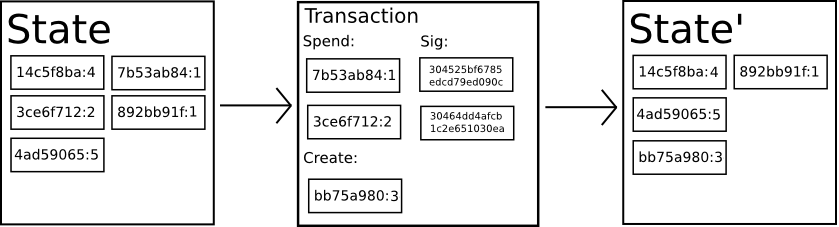
\includegraphics[width=1\linewidth]{Figures/BTC_statetransition_ETH_white_paper}
\decoRule
\caption{Bitcoin Zustandsveränderung durch Transaktion}
\label{fig:BTC_statetransition_ETH_white_paper}
\end{figure}

Die Transaktion aus Abbildung \ref{fig:BTC_statetransition_ETH_white_paper} überweist 1 Bitcoin von der Adresse \code{7b53ab84} und 2 Bitcoin von Adresse \code{3ce6f712} auf die Adresse \code{bb75a980} und überführt somit das Kontobuch in einen neuen Zustand. Möchten mehrere Teilnehmer den Systemzustand durch Transaktionen gleichzeitig anpassen, spielt die Reihenfolge in der die Transaktionen ausgeführt werden eine wichtige Rolle. Transaktionen werden in sogenannten Blöcken, in einer festen Reihenfolge, aggregiert. Somit werden nicht einzelne Transaktionen, sondern ganze Blöcke von Transaktionen in die Datenbank geschrieben. Genau wie bei den Transaktionen gibt es auch für Blöcke gewisse Konsensregeln. Sobald ein Block allen Konsensregeln entspricht, ist er bereit in die Datenbank aufgenommen zu werden.
Da sich alle Netzwerkteilnehmer über die Gültigkeit des Blockes einig sind, wird somit die globale Blockchain Datenbank angepasst. Genau wie bei den Transaktionen ist auch die Reihenfolge der Blöcke wichtig. Daher beinhaltet jeder Block den Hash-Wert seines Vorgängers(siehe \ref{fig:blockchain_ETH_white_paper}).

\begin{figure}[H]
\centering
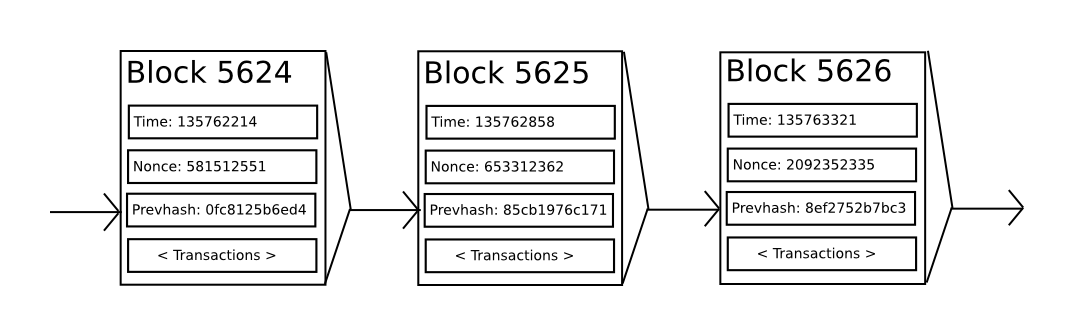
\includegraphics[width=1\linewidth]{Figures/blockchain_ETH_white_paper}
\decoRule
\caption[Kette von Blöcken]{Verkettung von Blöcken.}
\label{fig:blockchain_ETH_white_paper}
\end{figure}

Durch die so erzielte Verkettung der Blöcke wird die Reihenfolge eindeutig festgelegt und es entsteht die sogenannte Blockchain. Am Anfang der Blockchain befindet sich der sogenannte Genesis Block. Auf diesen bauen alle weiteren Blöcke auf. Nachträgliche Änderungen an einem bereits eingefügtem Block sind nicht möglich, da sich dadurch der Blockhash des Blocks verändert und somit an dieser Stelle die Kette ''zerbricht''.

\subsection{Konsensregeln}

Konsenzregeln sind Regeln über die sich alle Teilnehmer des Peer-to-Peer-Netzwerks einig sind. Sie stellen sicher, dass die grundlegenden Eigenschaften der Kryptowährung eingehalten werden. 
\if
Protokollregeln legen die Syntax der ausgetauschten Nachrichten fest. Konsensregeln legen dagegen die Semantik der ausgetauschten Nachrichten fest. 
Konsensregeln sind den Protokollregeln übergeordnet. Dies bedeutet, dass eine laut Protokollregeln korrekt aufgebaute Transaktionsnachricht, dennoch eine ungültige Transaktion enthalten kann, die den Konsensregeln widerspricht.
\fi
Bei Bitcoin gibt es eine ganze Reihe an Konsensregeln. Die wichtigsten sind:
\begin{itemize}
\item Transaktionen dürfen kein Geld aus dem nichts schöpfen, sondern nur bereits existierende Beträge von einer Adresse auf eine andere Adresse überweisen. Die Blockreward-Konsensregel bildet hierzu die einzige Ausnahme. Sie legt fest wie neue Währungseinheiten erschaffen werden.
\item Blockreward: Ein neuer Block muss genau eine Transaktion enthalten, die neue Kryptowährungseinheiten aus dem nichts erschafft. Sowohl die Höhe des Betrags als auch die Anpassung des Betrags über die Zeit ist in den Konsensregeln des Protokolls hart verankert. Bei Bitcoin startete der Blockreward bei 50 Bitcoin und halbiert sich seitdem alle 4 Jahre. Dies stellt sicher, dass es eine feste Obergrenze an Währungseinheiten gibt.
\item Transaktionen, die Geld von Adresse A nach Adresse B überweisen, müssen durch eine Signatur beweisen, dass sie von dem rechtmäßigen Besitzer getätigt werden.
\item Blockgröße: Diese Konsensregel legt die maximale Größe eines Blocks in Megabyte fest. Sie beeinflusst wie viele Transaktionen in einem Block gebündelt werden können. Dies ist wichtig, da sie zusammen mit der Blockzeit-Konsensregel das Wachstum der Blockchain-Datenbank steuert.
\item Blockzeit: Diese legt fest in welchem durchschnittlich Zeitabstand es erlaubt ist einen neuen Block in die Blockhain einzufügen. Bei Bitcoin ist diese Zeit auf 10 Minuten festgelegt.
\item Längste Blockchain-Kette: Teilnehmer des Peer-to-Peer Netzwerks folgen immer der Kette, die am meisten Proof-of-Work beinhaltet und betrachten ''kürzere'' Ketten als ungültig.
\end{itemize}
Die Konsensregeln ermöglichen es, dass jeder Teilnehmer eigenständig lokal seine Version der Blockchain Datenbank verwalten kann, ohne dabei einem anderen Teilnehmer vertrauen zu müssen. Die Konsensregeln stellen somit sicher, dass alle Teilnehmer die gleiche Blockchain Datenbank lokal aufbauen und sich dadurch auf den Systemzustand einigen.

\if Dadurch herrscht Einigkeit darüber welche Transaktionen bereits in die Blockchain aufgenommen wurden und somit als bestätigt gelten. Alle noch nicht in die Blockchain aufgenommen Transaktionen gelten als unbestätigt. \fi

\subsection{Proof-of-Work und Mining}
Das Einfügen eines neuen Blocks in die Blockchain Datenbank ist nur unter sehr strikten Regeln möglich. Bei einer dezentralen Währung wie Bitcoin gibt es keine zentrale Instanz, die solch eine Anpassung des Systemzustands koordiniert beziehungsweise autorisiert. Um dieses Problem zu lösen verwendet Bitcoin einen Proof-of-Work Algorithmus. Ziel des Algorithmus ist es durch das kontinuierliche\footnote{Das \code{nonce}-Feld des neusten Blocks wird nach jeder Berechnung des Hashwerts erhöht, damit ein neuer Hashwert entsteht.} Hashen des neusten Blocks einen Hashwert zu finden der unterhalb eines dynamisch angepassten Zielwerts liegt. Der Zielwert wird durch die Blockzeit Konsensregel so angepasst, dass im gesamten Netzwerk im Durchschnitt alle 10 Minuten ein neuer Bitcoin Block gefunden wird. Findet ein Teilnehmer den Blockhash eines den Konsensregeln entsprechenden Blocks, leitet er diesen Block an das Peer-to-Peer Netzwerk weiter und erhält im Gegenzug den Blockreward. Teilnehmer, die unbestätigte Transaktionen empfangen, diese in Blöcke zusammenfassen und unter Zuhilfenahme des Proof-of-Work Algorithmus in die Blockchain einfügen, werden ''Miner'' genannt. Dieser Name stammt daher, dass bei diesem rechenintensiven Prozess gleichzeitig neue Bitcoins erschaffen werden.

Beim Mining werden die in Tabelle \ref{tab:btc_block_header} aufgeführten Felder des Blockheaders als Eingabe für die kryptographische Hashfunktion SHA256 verwendet\footnote{Um genau zu sein wird der Blockheader bei Bitcoin zweimal mit der SHA 256 Hashfunktion gehasht. Blockhash = SHA256(SHA256(Blockheader))}.
\begin{table}[H]
\centering
\caption{Bitcoin Blockheader}
\label{tab:btc_block_header}
\begin{tabular}{|l|p{4,3cm}|p{4,3cm}|l|}
\hline
\textbf{Feld}  & \textbf{Verwendungszweck}                         & \textbf{Aktualisiert falls...}                                          & \textbf{Bytes} \\ \hline
version        & Block Versionsnumber                             & man die Software aktualisiert und diese eine neue Version spezifiziert. & 4              \\ \hline
hashPrevBlock  & 256-bit Hash des vorherigen Blockheaders          & ein neuer gültiger Block empfangen wird.                                & 32             \\ \hline
hashMerkleRoot & 256-bit Hash aller Transaktionen des Blocks       & eine neue Transaktion akzeptiert wird.                                  & 32             \\ \hline
time           & Aktueller Zeitstemple in Sekunden seit 1970-01-01 & Alle paar Sekunden...                                                   & 4              \\ \hline
bits           & Aktuelles Schwierigkeitsziel                      & wenn das Schwierigkeitsziel angepasst wird.                             & 4              \\ \hline
nonce          & 32-bit Nummer (von 0 aus erhöht)                  & der Hash ausprobiert wurde. (nonce+1)                                   & 4              \\ \hline
\end{tabular}
\end{table}
Die Transaktionen des Blocks gehen nicht direkt, nur durch den sogenannten Merkel Tree Hash\footnote{Der genaue Aufbau des Merkel Trees und dessen Vorteile sind in \cite{bitcoin_white_paper} genauer beschrieben.} in den Blockhash mit ein. Das \code{nonce}-Feld des Blockheaders wird nach jedem Hashversuch um den Wert 1 erhöht. Dadurch wird die Ausgabe der Hashfunktion kontinuierlich verändert.

Die Sicherheit des Bitcoin Netzwerkes und die Unmanipulierbarkeit der Blockchain ergeben sich aus der im Protokoll verankerten Spieltheorie. Die Spieltheorie macht es für einen Miner profitabler sich an die Spielregeln des Protokolls zu halten als zu versuchen das Netzwerk zu betrügen. Versucht ein Miner einen Block zu produzieren, der den Konsensregeln widerspricht, wird dieser vom Netzwerk verworfen. Somit hält kein anderer Netzwerkteilnehmer den vom Miner an sich selbst ausgeschütteten Blockreward für gültig. Da der Miner aber Ausgaben in Form von Hardwareabnutzung und Stromkosten zu bezahlen hat, schafft dies einen Anreiz sich den Konsensregeln zu unterwerfen. Solange 51 Prozent der Miner sich den Konsensregeln unterwerfen, formen diese auf Dauer die längste Blockchain. Die beim Mining anfallenden Stromkosten machen es außerdem sehr Teuer die Geschichte der Blockchain neu zu schreiben.
Das Mining ist ein sich selbst regulierendes System bei dem die Anzahl Miner\footnote{Genauer gesagt nicht die Anzahl Miner, sondern die von den Minern verwendete Rechenleistung.} sich mit dem Wert der Kryptowährung anpasst. Steigt der Preis pro Bitcoin, kommen neue Miner zum Netzwerk hinzu und machen das Netzwerk sicherer. Ein sinkender Preis hat zur Folge, dass der Blockreward nicht mehr für die Bezahlung der Strom und Hardwarekosten ausreicht. Dies hat zur Folge, dass die Anzahl an Miner abnimmt. Somit sinkt auch die Sicherheit des Netzwerks.